\documentclass{report}

\usepackage{my_lab}

\begin{document}

\LabTitle{3.2.3}{Резонанс токов в параллельном контуре}

% \tableofcontents
% \listoffigures
% \listoftables

\textbf{Цель работы}:
\begin{enumerate}
	\item исследование резонанса токов в параллельном колебатель­
	      ном контуре с изменяемой ёмкостью
	\item получение амплитудно-частотных и
	      фазово-частотных характеристик
	\item определение основных параметров кон­
	      тура
\end{enumerate}

\textbf{Приборы}:
\begin{enumerate}
	\item генератор сигналов
	\item источник напряжения, нагрузкой которого является параллельный
	      колебательный контур с пере­меннойёмкость
	\item двухканальный осциллограф
	\item цифровые вольтметры
\end{enumerate}

\section{Ход работы}
\begin{enumerate}
	\item Проведем настройку экспериментального стенда по техническому
	      описанию установки.

	\item Меняя частоту $ \nu $ генератора, убедимся по осциллографу и
	      вольтметрам, что у синусоиды $ U(t) $ меняется фаза и амплитуда,
	      тогда как синусоида  $ \mcE(t) $ привязана к началу координат:
	      $ \mcE(0) = 0,\ \dot{\mcE}(0) = 0 $.

	\item \label{p:3} Меняя $ C_n $ найдем резонансные частоты $ {\nu_0}_n $ и напряжения
	      $ U({\nu_0}_n) $. Резонанс можно найти по вольтметру или осциллографу.\\
	      См. таблицу \ref{table:1}.

	      \begin{table}[H]
		      \centering
		      \begin{tabular}{l|lll}
			        & $ \nu_0,\ \kilo\Hz $ & $ U,\ \Volt $ & $ E,\ \Volt $ \\
			      \hline
			      7 & 15.62                & 0.86          & 0.7143        \\
			      6 & 17.97                & 0.40          & 0.7142        \\
			      5 & 19.46                & 1.46          & 0.7144        \\
			      4 & 21.24                & 2.00          & 0.7145        \\
			      3 & 23.17                & 2.33          & 0.7145        \\
			      2 & 27.84                & 2.89          & 0.7145        \\
			      1 & 32.16                & 3.26          & 0.7144        \\
		      \end{tabular}
		      \caption{Измеренные значения п. \ref{p:3}}
		      \label{table:1}
	      \end{table}


	\item \label{p:4} Повторим измерения в п. \ref{p:3} при другом напряжении в
	      диапазоне $ 100 - 500\ \mili\Volt $.\\
	      См. таблицу \ref{table:2}.

	      \begin{table}[H]
		      \centering
		      \begin{tabular}{l|lll}
			        & $ \nu_0,\ \kilo\Hz $ & $ U,\ \Volt $ & $ E,\ \Volt $ \\
			      \hline
			      7 & 16.03                & 0.56          & 0.3587        \\
			      6 & 18.30                & 0.59          & 0.3586        \\
			      5 & 19.52                & 0.62          & 0.3586        \\
			      4 & 21.26                & 1.01          & 0.3587        \\
			      3 & 23.20                & 1.13          & 0.3587        \\
			      2 & 27.57                & 1.47          & 0.3588        \\
			      1 & 31.84                & 1.52          & 0.3588        \\
		      \end{tabular}
		      \caption{Измеренные значения п. \ref{p:4}}
		      \label{table:2}
	      \end{table}

	\item \label{p:5} Для двух разных $ C_n $ снимим АЧХ $ U(f) $ вблизи резонанса, при
	      $ U(f) \ge 0.6\ U(\nu_0) $ \\(18 точек по обе стороны).\\
	      См. таблицу \ref{table:3}.

	      \begin{table}[H]
		      \centering
		      \begin{tabular}{l|lll}
			              & $ \nu,\ \kilo\Hz $ & $ U,\ \Volt $ & $\Delta \psi, \pi$ \\
			      \hline
			      $ C_7 $ & 16.15              & 0.58          & 12.2               \\
			              & 16.35              & 0.50          & 10.6               \\
			              & 16.50              & 0.43          & 10.9               \\
			              & 16.65              & 0.41          & 8.0                \\
			              & 16.60              & 0.39          & 8.0                \\
			              & 16.70              & 0.35          & 9.0                \\
			              & 16.75              & 0.34          & 9.5                \\
			              & 16.01              & 0.59          & 1.4                \\
			              & 15.90              & 0.55          & 2.5                \\
			              & 15.80              & 0.52          & 4.5                \\
			              & 16.57              & 0.47          & 6.0                \\
			              & 15.33              & 0.40          & 8.0                \\
			              & 16.48              & 0.37          & 8.5                \\
			              &                    &               &                    \\
			      $ C_4 $ & 21.30              & 1.00          & 1.0                \\
			              & 21.40              & 0.96          & 2.0                \\
			              & 5.00               & 0.90          & 3.5                \\
			              & 6.00               & 0.82          & 4.5                \\
			              & 7.00               & 0.75          & 5.5                \\
			              & 8.00               & 0.58          & 6.6                \\
			              & 8.50               & 0.54          & 6.5                \\
			              & 2.00               & 0.99          & 0.7                \\
			              & 21.10              & 0.95          & 2.0                \\
			              & 21.00              & 0.88          & 3.5                \\
			              & 20.90              & 0.80          & 5.0                \\
			              & 20.80              & 0.72          & 6.0                \\
			              & 20.75              & 0.69          & 6.0                \\
			              & 20.70              & 0.65          & 6.5                \\
		      \end{tabular}
		      \caption{Измеренные значения п. \ref{p:5} и п. \ref{p:6}}
		      \label{table:3}\label{table:4}
	      \end{table}

	\item \label{p:6} Для техже $ C_n $ и $ \mcE $ из пункта \ref{p:5} измерим ФЧХ
	      $\psi_U(f) $ при $ U(f) \ge 0.3\ U(\nu_0) $.\\
	      См. таблицу \ref{table:4}.

	\item \label{p:7} Результаты п. \ref{p:3} пнесем в таблицу, как на рис. \ref{fig:table_example}.
	      См. таблицу \ref{table:5}.\\
	      \begin{figure}[H]
		      \centering
		      \def\svgwidth{\columnwidth}
		      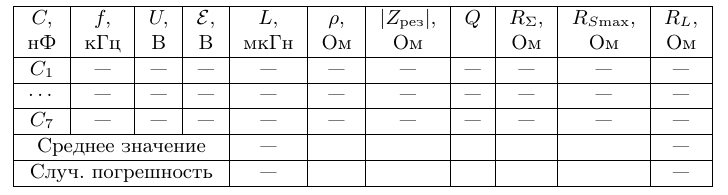
\includegraphics[scale = 0.6]{figures/table_example.png}
		      \caption{table\_example}
		      \label{fig:table_example}
	      \end{figure}
          \begin{gather}
              L=\frac{1}{C(2\pi f)^2} \\
              \rho=\frac{1}{2\pi fC} \\
              Z_{\text{рез}}=\frac{U}{E_0} R_1 \\
              Q= \frac{Z_{\text{рез}}}{\rho} = \frac{UR_1}{E_0}2\pi fC \\
              R_{\Sigma}= \frac{\rho^2}{Z_{\text{рез}}} \frac{E_0}{UR_1}\frac{1}{(2\pi fC)^2} \\
              R_{Smax} = \rho \tan{\delta} \approx 10^{-3}\cdot\frac{1}{\omega_0C} \\
              R_L = R_\Sigma - R_S - R = \frac{E_0}{UR_1}\frac{1}{(2\pi fC)^2}-R-10^{-3}\cdot\frac{1}{\omega_0C}
          \end{gather}
	      \begin{table}[H]
		      \centering
		      \begin{tabular}{l|lllllllllll}
			        & $ C,\ \nano\Farad $ & $ \nu_0,\ \kilo\Hz $ & $ U,\ \Volt $ & $ E,\ \Volt $ & L, мкГн & $ \rho,\ \Ohm $ & $ \abs{Z_{\text{рез}}},\ \Ohm $ & $ Q $ & $ R_\Sigma, \Ohm $ & $ {R_S}_{max}, \Ohm $ & $ R_L, \Ohm $ \\
			      \hline
			      7 & 101.5               & 15.62                & 0.86          & 0.7143        & 1023    & 100             & 1216                            & 12.1  & 8.3                & 0.10                  & 4.69          \\
			      6 & 82.7                & 17.97                & 1.16          & 0.7142        & 949     & 107             & 1638                            & 15.3  & 7.0                & 0.11                  & 6.89          \\
			      5 & 67.5                & 19.46                & 1.46          & 0.7144        & 991     & 121             & 2060                            & 17.0  & 7.1                & 0.12                  & 7.01          \\
			      4 & 57.4                & 21.24                & 2.00          & 0.7145        & 978     & 131             & 2814                            & 21.6  & 6.1                & 0.13                  & 5.92          \\
			      3 & 47.3                & 23.17                & 2.33          & 0.7145        & 998     & 145             & 3289                            & 22.6  & 6.4                & 0.15                  & 6.27          \\
			      2 & 32.3                & 27.84                & 2.89          & 0.7145        & 1012    & 177             & 4078                            & 23.0  & 7.7                & 0.18                  & 7.50          \\
			      1 & 25.1                & 32.16                & 3.26          & 0.7144        & 976     & 197             & 4606                            & 23.4  & 8.4                & 0.20                  & 8.24          \\
			      \hline
			        &                     &                      &               &               & 989     &                 &                                 &       &                    &                       & 6.65          \\
			        &                     &                      &               &               & 61      &                 &                                 &       &                    &                       & 2.83          \\
		      \end{tabular}
		      \caption{Измеренные значения п. \ref{p:7}}
		      \label{table:5}
	      \end{table}

	      Получили, что\\
	      \begin{gather}
		      L = (989 \pm 61)\ \micro\Henry \\
		      R_L = (6.65 \pm 2.83)\ \Ohm
	      \end{gather}

	\item \label{p:8} Выполним п. \ref{p:7} по результатам п. \ref{p:4}.
	      См. таблицу \ref{table:6}.\\
	      \begin{table}[H]
		      \centering
		      \begin{tabular}{l|lllllllllll}
			        & $ C,\ \nano\Farad $ & $ \nu_0,\ \kilo\Hz $ & $ U,\ \Volt $ & $ E,\ \Volt $ & L, мкГн & $ \rho,\ \Ohm $ & $ \abs{Z_{\text{рез}}},\ \Ohm $ & $ Q $ & $ R_\Sigma, \Ohm $ & $ {R_S}_{max}, \Ohm $ & $ R_L, \Ohm $ \\
			      \hline
			      7 & 101.5               & 16.03                & 0.56          & 0.3587        & 971     & 98              & 1561                            & 16.0  & 6.1                & 0.10                  & 6.03          \\
			      6 & 82.7                & 18.30                & 0.59          & 0.3586        & 915     & 105             & 1664                            & 15.8  & 6.6                & 0.11                  & 6.54          \\
			      5 & 67.5                & 19.52                & 0.62          & 0.3586        & 985     & 121             & 1751                            & 14.5  & 8.3                & 0.12                  & 8.21          \\
			      4 & 57.4                & 21.26                & 1.01          & 0.3587        & 976     & 130             & 2831                            & 21.7  & 6.0                & 0.13                  & 5.88          \\
			      3 & 47.3                & 23.20                & 1.13          & 0.3587        & 995     & 145             & 3175                            & 21.9  & 6.6                & 0.15                  & 6.48          \\
			      2 & 32.3                & 27.57                & 1.47          & 0.3588        & 1032    & 179             & 4137                            & 23.1  & 7.7                & 0.18                  & 7.54          \\
			      1 & 25.1                & 31.84                & 1.52          & 0.3588        & 995     & 199             & 4282                            & 21.5  & 9.3                & 0.20                  & 9.06          \\
			        &                     &                      &               &               & 981     &                 &                                 &       &                    &                       & 7.11          \\
			        &                     &                      &               &               & 87      &                 &                                 &       &                    &                       & 2.93          \\
		      \end{tabular}
		      \caption{Измеренные значения п. \ref{p:8}}
		      \label{table:6}
	      \end{table}
	      Получили, что\\
	      \begin{gather}
		      L = (981 \pm 87)\ \micro\Henry \\
		      R_L = (7.11 \pm 2.93)\ \Ohm
	      \end{gather}

	      Значения L довольно близки, в пределах погрешности. Случайная погрешность не велика.
	      $ R_L $ значительно отличаются, но в пределах погрешности.Случайная погрешность $ R_L $ велика.

	\item По данным из п. \ref{p:5} построим графики $ U(\nu) $. Проведем анализ характеристик.\\
	      См. рис. \ref{fig:U}.
	      \begin{figure}[H]
		      \centering
		      \def\svgwidth{\columnwidth}
		      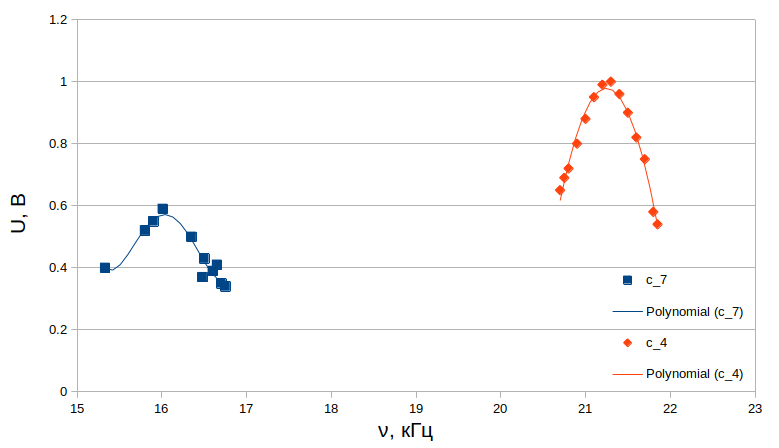
\includegraphics[scale = 0.6]{figures/U3.png}
		      \caption{$U(\nu)$}
		      \label{fig:U}
	      \end{figure}
	      % TODO:

	\item \label{p:10} По данным из п. \ref{p:5} построим графики в безразмерных координатах:
	      $ x = \frac{\nu}{\nu_0},\ y = \frac{U}{U(\nu_0)} $. Проведем анализ характеристик.\\
	      См. рис. \ref{fig:U2}.
	      \begin{figure}[H]
		      \centering
		      \def\svgwidth{\columnwidth}
		      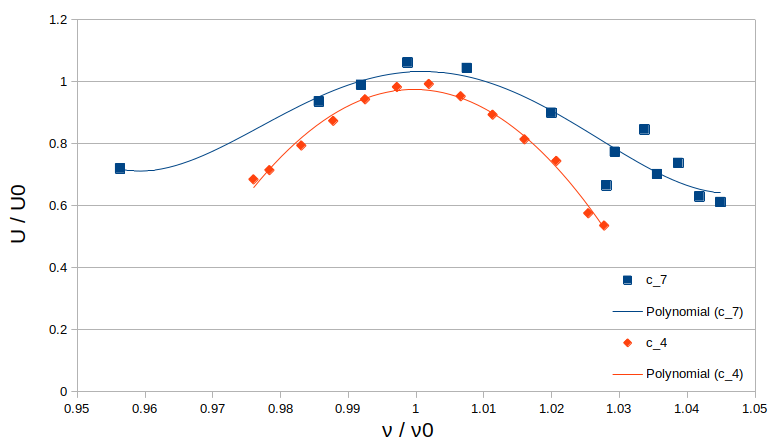
\includegraphics[scale = 0.6]{figures/F.png}
		      \caption{$\frac{U}{U_0}(\frac{\nu}{\nu_0})$}
		      \label{fig:U2}
	      \end{figure}
	      % TODO:

	\item По данным из п. \ref{p:6} построим графики в координатах:
	      $ x = \frac{\nu}{\nu_0},\ y = \frac{\psi_U}{\pi} $. Проведем анализ характеристик.\\
	      См. рис. \ref{fig:psi}.\\
	      \begin{figure}[H]
		      \centering
		      \def\svgwidth{\columnwidth}
		      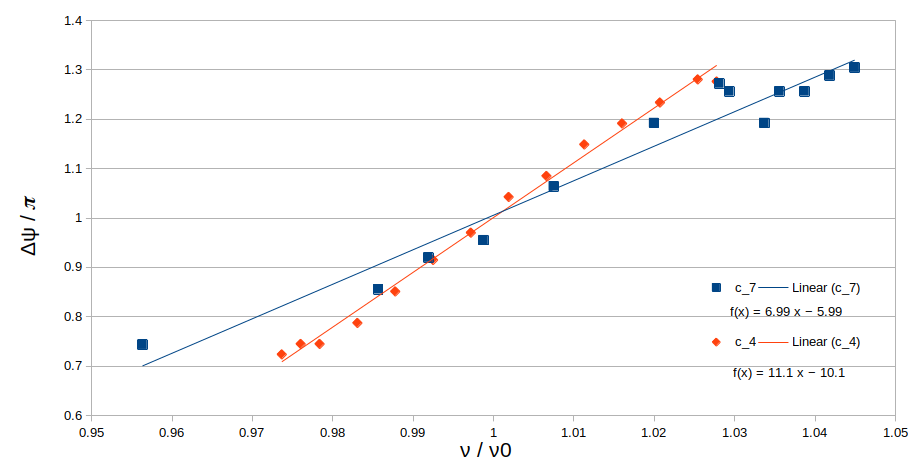
\includegraphics[scale = 0.5]{figures/Psi2.png}
		      \caption{$\frac{U}{U_0}(\frac{\nu}{\nu_0})$}
		      \label{fig:psi}
	      \end{figure}
	      По характеристикам определим добротности контуров двумя способами:\\
	      1. $ Q = \frac{1}{2} \dv{x}{\psi_U}(1) $\\
	      $ Q = \frac{\pi}{2} \dv{x}{y} $\\
	      $ C_4: \dv{x}{y} \approx 11.1 $\\
	      $ C_7: \dv{x}{y} \approx 9.2 $\\
	      \begin{gather}
		      Q_4 \approx 17.4 \\
		      Q_7 \approx 14.5 \\
	      \end{gather}
	      \\
	      % TODO: understand

	      % 2. По расстоянию $ \frac{1}{Q} $ между точками оси x, в которых
	      % меняется от $ -\frac{1}{4} $ до $ \frac{1}{4} $.\\
	      % Оценим погрешности.\\
	      % Сравним с результатами из п. \ref{p:7} и п. \ref{p:10}.

	      Значения $ Q $ близки к полученным в п. \ref{p:8}:\\
	      \begin{gather}
		      Q_4 \approx 21.7 \\
		      Q_7 \approx 16.0 \\
	      \end{gather}

	\item Построим зависимость $ R_L({\nu_{0}}_n) $ в системе координат с началом в
	      точке $ (0.6\cdot {\nu_0}_7;\ 0) $. Построим прямую $ y = \avrg{R_L} $.\\
	      См. рис. \ref{fig:RL}.\\
	      Назовем возможные причины изменения $ R_L $.
	      \begin{figure}[H]
		      \centering
		      \def\svgwidth{\columnwidth}
		      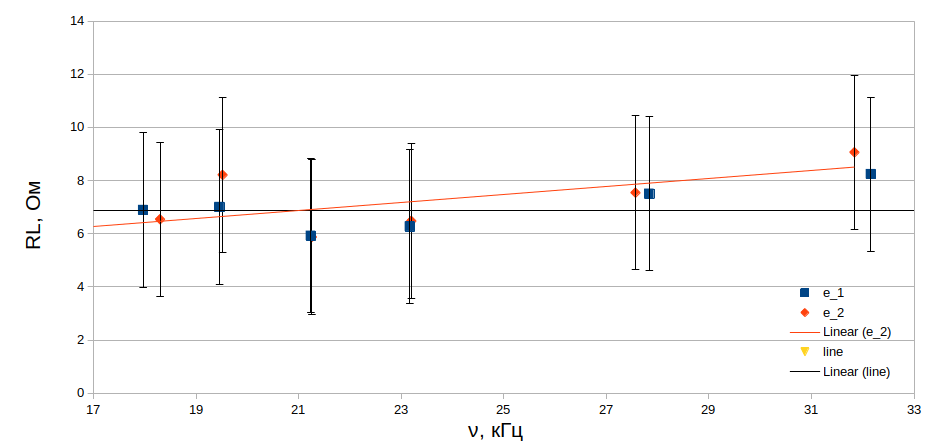
\includegraphics[scale = 0.5]{figures/RL.png}
		      \caption{ $ R_L(\nu_0) $ }
		      \label{fig:RL}
	      \end{figure}

	      Можно заметить, что $ R_L $ медленно возростает с частотой.\\

	\item Построим векторную диаграмму токов и напряжений для контура с
	      наименьшей добротностью в резонансном состоянии.\\
	      % См. рис. \ref{fig:f}.\\

	      % TODO: understand

\end{enumerate}

\section{Вывод.}

В данной работе мы изучили резонанс токов в параллельном контуре.
Меняя состояние цепи, нашли резонансы. По полученным измерениям нашли
индуктивность катушки $ L $, $ R_L $ и добротность $ Q $.
Мы построили графики АЧХ и ФЧХ. Оценили добротность по графикам и получили схожие результаты.

\end{document}
